%\documentclass{article}
%\usepackage{tikz,pgfplots}
%\usepackage[pdftex,active,tightpage]{preview}
%\begin{document}
%\begin{preview}
%%%%%%%%%%%%%%%%%%%%%%%%%%%%%%
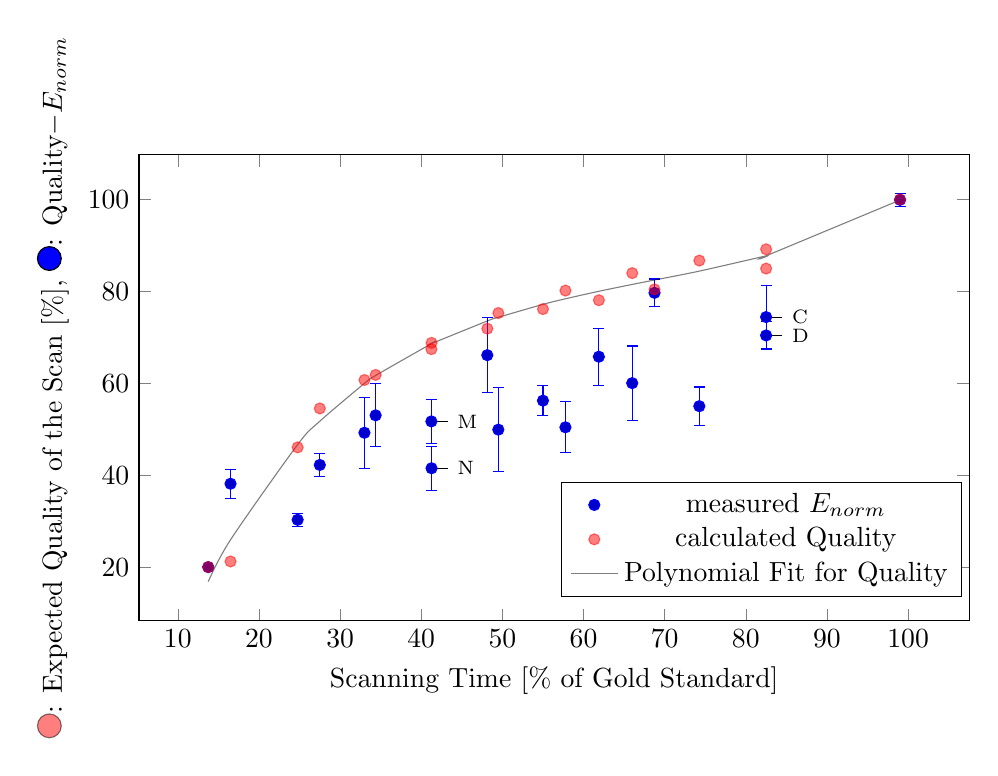
\begin{tikzpicture}

\begin{axis}[%
	width=\linewidth,
	height=0.618\linewidth,
%%%%%%%%	scale only axis,
%%%%%%%%	xmin=0,xmax=110,
%%%%%%%%	ymin=0,ymax=110,
%%%%%%%%	axis y line = left,
	xlabel={Scanning Time [\%\ of Gold Standard]},%
	ylabel={%
		\tikz \draw[fill=red,semitransparent] (0ex,0ex) circle (1ex);: %
		Expected Quality of the Scan [\%], %
		\tikz \draw[fill=blue] (0ex,0ex) circle (1ex);: %
		Quality$-E_{norm}$%
		}%
	]

\addplot
plot [ only marks,
	error bars/.cd,
    y dir=both,y explicit ]
    coordinates{
	(13.75,20.0000) +- (0,0)      % T
	(16.50,38.1358) +- (0,3.1135) % S
	(24.77,30.2919) +- (0,1.3958) % R
	(27.50,42.2255) +- (0,2.5278) % Q
	(33.00,49.2247) +- (0,7.6789) % P
	(34.38,53.0181) +- (0,6.8507) % O 
	(41.27,41.5079) +- (0,4.7824) % N  
	(41.25,51.6990) +- (0,4.7110) % M
	(49.50,49.9058) +- (0,9.1839) % L
	(48.14,66.1100) +- (0,8.1635) % K
	(57.77,50.4137) +- (0,5.5671) % J
	(55.00,56.2138) +- (0,3.2329) % I
	(66.00,60.0243) +- (0,8.0805) % H
	(61.89,65.7727) +- (0,6.2214) % H
	(74.27,55.0069) +- (0,4.1882) % F
	(68.75,79.6708) +- (0,3.0107) % E
	(82.50,70.4018) +- (0,3.0863) % D
	(82.50,74.3991) +- (0,6.8125) % C
	(99.01,99.8987) +- (0,1.3487) % B
	};

% Protocols
\addplot [ color = red, semitransparent, only marks, mark = *]
	coordinates{
		(13.7508,20)
		(16.5009,21.2284)
		(24.7703,46.0522)
		(27.5016,54.5201)
		(33.0019,60.7072)
		(34.3801,61.8107)
		(41.2524,67.4167)
		(41.2712,68.7811)
		(48.1435,71.8724)
		(49.5028,75.28)
		(55.0031,76.1345)
		(57.7722,80.1592)
		(61.8943,78.0612)
		(66.0038,83.9645)
		(68.7539,80.4284)
		(74.2731,86.6889)
		(82.5047,84.9458)
		(82.5047,89.1421)
		(99.0057,100)
};

% Line plot
\addplot [smooth, solid, semitransparent]
	coordinates{
		(13.7508,16.8548)
		(16.5009,25.9575)
		(24.7703,46.6567)
		(27.5016,51.7347)
		(33.0019,59.9714)
		(34.3801,61.6854) 
		(41.2524,68.6146)
		(41.2712,68.6305) 
		(48.1435,73.5452)
		(49.5028,74.3455)
		(55.0031,77.1605)
		(57.7722,78.3754)
		(61.8943,80.0091)
		(66.0038,81.5005)
		(68.7539,82.4599)
		(74.2731,84.3973)
		(82.5047,87.719)
		(82.5047,87.719)
		(99.0057,99.8565)
};

\pgfplotsset{every axis legend/.append style={at={(0.75,0.1)},anchor=base}}

\legend{measured $E_{norm}$,calculated Quality, Polynomial Fit for Quality}

\draw [] (axis cs:82.50,74.3991) -- (axis cs:84.50,74.3991) node [right] {\scriptsize C};
\draw [] (axis cs:82.50,70.4018) -- (axis cs:84.50,70.4018) node [right] {\scriptsize D};
\draw [] (axis cs:41.25,51.6990) -- (axis cs:43.25,51.6990) node [right] {\scriptsize M};
\draw [] (axis cs:41.27,41.5079) -- (axis cs:43.27,41.5079) node [right] {\scriptsize N};

\end{axis}

\end{tikzpicture}
%%%%%%%%%%%%%%%%%%%%%%%%%%%%%%
% plot erstellt mit MATLAB-File p:\\MATLAB\WideFieldScan/Paper/wfs_Compare2008c_ErrorPlot.m
% mit FromToTo = 1:5:1024
% sowie matlab2tikz
% Daten
%%%%%%%%%%Time =
%%%%%%%%%%  Columns 1 through 12
%%%%%%%%%%
%%%%%%%%%%   13.75   16.50   24.77   27.50   33   34.38   41.27   41.25   49.50   48.14   57.77   55
%%%%%%%%%%
%%%%%%%%%%  Columns 13 through 19
%%%%%%%%%%
%%%%%%%%%%   66   61.89   74.27   68.75   82.50   82.50   99.01
%MeanCumulativeError =
%
%  Columns 1 through 12
%
%   20.0000   38.1358   30.2919   42.2255   49.2247   53.0181   41.5079   51.6990   49.9058   66.1100   50.4137   56.2138
%
%  Columns 13 through 19
%
%   60.0243   65.7727   55.0069   79.6708   70.4018   74.3991   99.8987
%
%
%StandardDeviationofCumulativeError =
%
%  Columns 1 through 12
%
%         0    3.1135    1.3958    2.5278    7.6789    6.8507    4.7824    4.7110    9.1839    8.1635    5.5671    3.2329
%
%  Columns 13 through 19
%
%    8.0805    6.2214    4.1882    3.0107    3.0863    6.8125    1.3487
%%%%%%%%%%%%%%%%%%%%%%%%%%%%%%
%\end{preview}
%\end{document}